\clearpage
\bigsection{Evaluation}
To evaluate our work, we run our analyses on various applications and also run benchmarks to compare the performance before and after using profile-guided optimizations.
As we need Vulkan applications, we picked the following five games:
Ashes of the Singularity which we will sometimes abbreviate as \emph{Ashes} in the following, Dota 2, F1 2017, Mad Max and Warhammer 40,000: Dawn of War III which we will shorten to Warhammer.
We also looked at Vulkan benchmarks like vkmark, but this tool does not focus on shaders but instead on the rest of the graphics pipeline.
Therefore, the shaders are simple and do not provide possibilities for PGO. E.g. using the default LLVM PGO on the shaders did not change a single instruction.
The selected games have in common that they use the Vulkan API on Linux, and they have a benchmark which can be executed automatically and collects the performance data in a machine-readable form.
There are similar games, which we tried to use but failed because of various problems, like the game does not start at all under Linux.
The games that we excluded are F1 2018, Serious Sam Fusion 2017 and Total War Saga: Thrones of Britannia, which was not even installable through Steam.

Another game focused application which we looked at is the Infiltrator Demo Project of the Unreal Engine~\cite{Games2015}.
This is not a real game, but a demo scene is played when the application starts to showcase the game engine.
Also, it does not measure the performance to our knowledge, so we did not use it to test the performance of PGO, but we measured the amount of needed registers.
Another non-game application which we used for evaluation purpose is a small switch-case bytecode interpreter that we will describe further in \cref{sub:eval_unused}.
In total, more than $6 \frac{1}{2}\;\si{h}$ was spent running benchmarks.

The performance numbers are expressed as frame times, i.e. how long does it take to compute a single frame for the game.
For example a frame time of \SI{16.6}{\milli\second} roughly corresponds to 60 frames per second.
The lower the frame time is, the more pictures are shown per second and the better is the performance.
The measured times are always given with a standard error using a confidence level of \SI{68.3}{\percent} with the Student's t-distribution.

An application like a game uses a lot of shaders, Ashes has 250 different shaders, Dota 2 compiles 877 shaders for the benchmark scene and Mad Max 734 shaders.
Warhammer uses the least amount with 225 shaders while F1 2017 needs the most with 3220.
These numbers do not necessarily represent the total number of shaders in the games, but only the amount of shaders which are compiled for the benchmark scene.
A difference here is that Ashes compiles most of its shaders at the start of the game while Dota compiles shaders lazily when they are needed, so we only saw a fraction of the shaders that Dota contains, but we saw a greater fraction of the shaders in Ashes.
When evaluating basic block counters, unused code and uniformity, we only consider shaders which were run at least once.
For the register usage, we collect the statistics over all compiled shaders without taking into account if they have been needed or not.

\subsection{Basic Block Counters}
\label{sub:eval_counters}
Shaders are small programs compared to CPU programs, more like a single function.
This means the number of basic blocks in a shader is low, usually around 20 or lower.
After instrumenting the shaders and running a benchmark, we have a counter associated with each basic block which tells us how often each block was executed.

LLVM uses the counters e.g. for linearization. A performance comparison using the default optimizations in LLVM that rely on PGO data is discussed in \cref{sub:eval_perf}.
An additional effect of PGO apart from linearization which can be observed when instrumenting before the \texttt{StructurizeCFG} pass is that most pixel shaders are marked as hot functions while vertex shaders are often marked as unlikely.
The reason is that a triangle contains three vertices but a lot more pixels.
Hence a pixel shader gets executed more often than a vertex shader and LLVM marks them accordingly.

To get an intuition for the collected counter values, we visualize them in a few diagrams.
\Cref{dia:counter_values} shows a histogram of the basic blocks, sorted by execution count.
The x-axis of this diagram represents the counter, i.e. how often a basic block is executed.
A bar for the execution counts $0.8\cdot 10^{12}--1.2\cdot 10^{12}$ for example represents all blocks which get run at least $0.8\cdot 10^{12}$ times but less than $1.2\cdot 10^{12}$ times.
The height of the bar counts how many basic blocks fall into this range, in this example one basic block of all shaders in Dota 2 falls into the range.
The lowest bucket of the diagram, the leftmost bar, contains most of the blocks.
This bar is cut off, otherwise the rest of the bars would not be visible.
This means most basic blocks get executed less than $10^10$ times.
A few blocks run a lot more often, two of them more than $10^{12}$ times.
The blocks that are run most often are the inner parts of a hot loop in a shader.
\begin{figure}
\pgfplotsset{width=\textwidth}
\centering
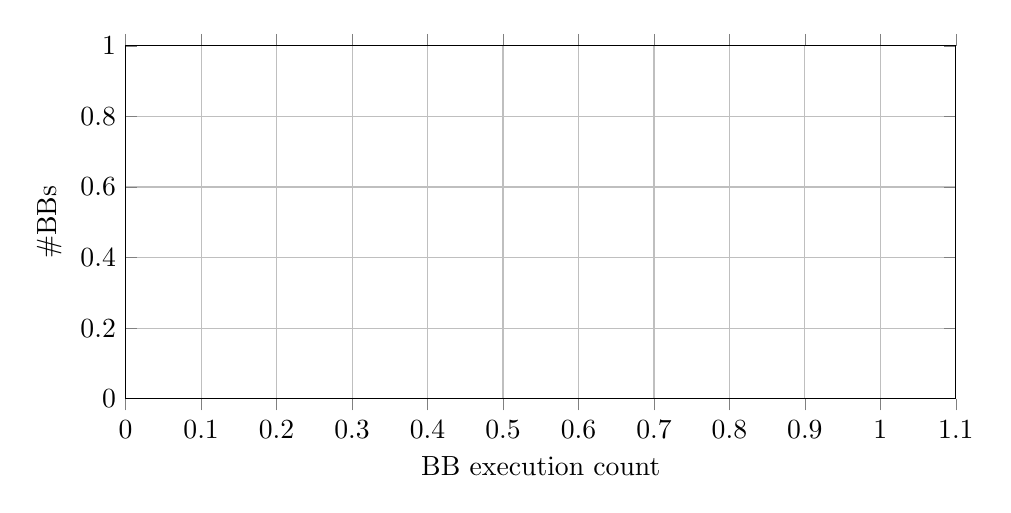
\begin{tikzpicture}
\begin{axis}[
	ybar,
	xlabel={BB execution count},
	ylabel={\#BBs},
	xmin=0,
	ymin=0,
	ymax=20,
	grid=both,
	%bar width=0.5cm,
]

\runtex{counter-dist1 -g dota}

\node at (axis cs:15e9,19) {\color{white}↑};
\end{axis}
\end{tikzpicture}
\captionof{figure}{The distribution of counter values on basic blocks of Dota 2}
\label{dia:counter_values}
\end{figure}


\Cref{dia:counter_values2} gives a detailed view of the leftmost part of \cref{dia:counter_values}.
It only shows the range up to $10^5$ executions.
In this range, the blocks are distributed more equal, still we see that most blocks are executed seldom while blocks with a higher counter value are rare.
\begin{figure}
\pgfplotsset{width=\textwidth}
\centering
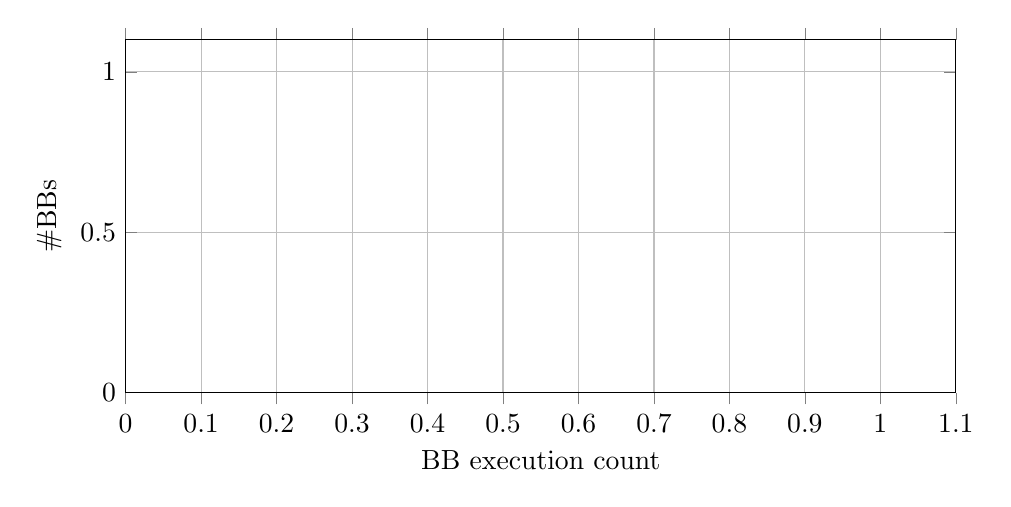
\begin{tikzpicture}
\begin{axis}[
	ybar,
	xlabel={BB execution count},
	ylabel={\#BBs},
	xmin=0,
	ymin=0,
	grid=both,
	%bar width=0.5cm,
]

\runtex{counter-dist2 -g dota}
\end{axis}
\end{tikzpicture}
\captionof{figure}{The distribution of counter values on basic blocks of Dota 2}
\label{dia:counter_values}
\end{figure}


%TODO
Ashes as of 2019-09-01 shows graphical artifacts when using PGO.
This hints that there is a bug in LLVM that only gets triggered when profile-guided optimizations are enabled.

\subsection{Unused code}
\label{sub:eval_unused}
Looking at basic blocks which get never executed, we can remove them and study the changes in register usage and performance.
The performance comparison can be found in \cref{sub:eval_perf}, this section shows statistics about the amount of unused code.
The fraction of unused basic blocks ranges from \SI{0.22}{\percent} in Mad Max up to \SI{37.46}{\percent} unused blocks in in Warhammer.
\Cref{dia:unused_by_game} shows a comparison of all analyzed games.
\begin{figure}
\pgfplotsset{width=\textwidth}
\centering
\begin{tikzpicture}
\runtex{unused-code-summary}
\end{tikzpicture}
\captionof{figure}{The fraction of unused basic blocks per game}
\label{dia:unused_by_game}
\end{figure}


To gain more insight into how shaders and the unused code is distributed, \Cref{dia:unused_by_bb_ashes} and following show the unused code with respect to the size of a shader in basic blocks.
The x-axis represents the size of a shader, the amount of blocks that a shader contains.
The gray plot in the background displays the distribution of all shaders in an application.
A height of \SI{6}{\percent} at one point (the right y-axis is the crucial one here) means that about \SI{6}{\percent} of all shaders in the game have this amount of basic blocks.
Each black line represents a shader with unused code. The left y-axis is connected to the percentage of unused code.
\newcommand\unuseddiag[2]{
\begin{figure}
\pgfplotsset{width=\textwidth,height=7cm}
\centering
\begin{tikzpicture}
\begin{axis}[
	ybar,
	xlabel={\#BBs in a Shader},
	ylabel={Unused BBs [\SI{}{\percent}]},
	xmin=0,
	xmax=\runtex{max-bbs -g #1},
	ymin=0,
	ymax=100,
	ytick pos=left,
	grid=both,
	bar width=0.01cm,
]

\runtex{unused-code -g #1}
\end{axis}

\begin{axis}[
	axis y line*=right,
	axis x line=none,
	xlabel={\#BBs in a Shader},
	ylabel={Distribution of shaders [\SI{}{\percent}]},
	xmin=0,
	xmax=\runtex{max-bbs -g #1},
	ymin=0,
	legend style={at={(1,1)},anchor=north east},
]
\addlegendimage{only marks, fill=gray, draw=gray, fill opacity=0.4}\addlegendentry{Shader distribution}
\runtex{bbs -g #1}
\addlegendentry{Shader with unused BBs}
\end{axis}
\end{tikzpicture}
\captionof{figure}{The fraction of unused code by shader size in #2}
\label{dia:unused_by_bb_#1}
\end{figure}
}

\unuseddiag{ashes}{Ashes}
\unuseddiag{dota}{Dota 2}
\unuseddiag{f12017}{F1 2017}
\unuseddiag{madmax}{Mad Max}
\unuseddiag{dow3}{Warhammer}
\unuseddiag{switch}{the switch vm}


We test the effect of removing unused code on the games Dota 2 and Mad Max and on a small sample program.
Our code to remove basic blocks is not robust enough to work for all tested games and only Dota 2 and Mad Max ran flawlessly, thus the other games were not benchmarked in this configuration.
The small sample program runs a bytecode virtual machine in a shader using one large switch-case statement.
Each case statement contains the code for one virtual instruction and the shader iterates through every instruction.
The bytecode in our benchmark runs uses only a single instruction out of the 71 possible instructions.
The code is transferred to the shader through a uniform buffer, consists of 128 instructions stored in \SI{4}{\kibi\byte} of memory and is executed two times until the result is used as the final fragment color.
LLVM compiles the switch statement into a binary jump tree, therefore in each iteration of the virtual machine, multiple jumps are executed until the right case for the current instruction is found.

Using PGO, we detect that all instructions in all but one case statements are never executed.
Thus, in the optimized shader version we can remove all these basic blocks.
This leaves us with compare and jump instructions from the original binary jump tree but only one of the branch instructions is taken and the code has fewer basic blocks than before.
This improves the performance as seen in \cref{sub:eval_perf}.

Apart from performance, we also want to analyze the register usage of shaders when removing unused blocks.
This can help us to estimate gains of register spilling to reduce register pressure.
When looking at registers, we have to differentiate between scalar and vector registers.
Scalar registers are cheap in hardware compared to vector registers because we only need $\frac{1}{64}$ of them.
Hence, we have more of them and the occupancy of shaders is mostly limited by vector registers.
We also split our observations by shader type, we look at compute, vertex and pixel/fragment shaders separately.
Each game is tested in three configurations: Running the game without any special options, using profile-guided optimizations and using PGO with removing unused basic blocks.
The figures starting at \cref{dia:registers_cs-vgpr} show the register usage, averaged over all shaders that fall into the category, e.g. vector registers in compute shaders in the first diagram.
\newcommand\regusage[4]{
\begin{figure}
\pgfplotsset{width=\textwidth}
\centering
\begin{tikzpicture}
\begin{axis}[
	ybar,
	enlarge x limits=0.2,
	cycle list name=mycolors,
	symbolic x coords={ashes,dota,dow3,f12017,infiltrator,madmax},
	xticklabels={Ashes,Dota 2,Warhammer,F1 2017,Unreal Infiltrator,Mad Max},
	xtick=data,
	xticklabel style={text width=2cm,align=center},
	ylabel={\#Registers used},
	ymin=0,
	ymax=#4,
	grid=both,
	nodes near coords,
	every node near coord/.append style={rotate=90, anchor=west},
	bar width=0.5cm,
	legend style={at={(0,1)},anchor=north west},
]

\runtex{registers -g #1}
\end{axis}
\end{tikzpicture}
\captionof{figure}{#3 usage in #2}
\label{dia:registers_#1}
\end{figure}
}

\regusage{cs-vgpr}{compute shaders}{Average vector register}{65}
\regusage{cs-sgpr}{compute shaders}{Average scalar register}{65}
\regusage{vs-vgpr}{vertex shaders}{Average vector register}{60}
\regusage{vs-sgpr}{vertex shaders}{Average scalar register}{80}
\regusage{ps-vgpr}{pixel shaders}{Average vector register}{75}
\regusage{ps-sgpr}{pixel shaders}{Average scalar register}{125}


The average register usage stays the same when using PGO. Ashes sometimes uses a bit fewer registers than normal, F1 2017 sometimes more but the differences are small.
Mad Max shows the greatest effect when removing unused code, it sometimes reduces the register usage by one register on average.
A more detailed analysis of the effect of removing unused blocks in \cref{dia:registers_scatter} shows the register amount for each shader before and after removing blocks.
Every dot represents a shader, the x-coordinate is the amount of used registers when compiling the shader with PGO, the y-coordinate are the registers when compiling with PGO and additionally removing blocks which never get executed.
Most shaders lie on the diagonal, which means the amount of registers does not change.
A few points are above the diagonal, so the compiler allocates more registers for them when unused code is removed.
Some points are also below the diagonal, meaning they need fewer registers when blocks are removed.
Mad Max uses a pixel shader with a lot of computations, but these computations never get executed in the benchmarks.
Thus, when removing unused basic blocks, only a simple shader that checks an always false condition remains and fewer vector registers are used.
This shader can be seen in the lower right corner of \cref{dia:registers_scatter}.
\begin{figure}
\pgfplotsset{width=0.5\textwidth,height=0.5\textwidth}
\centering
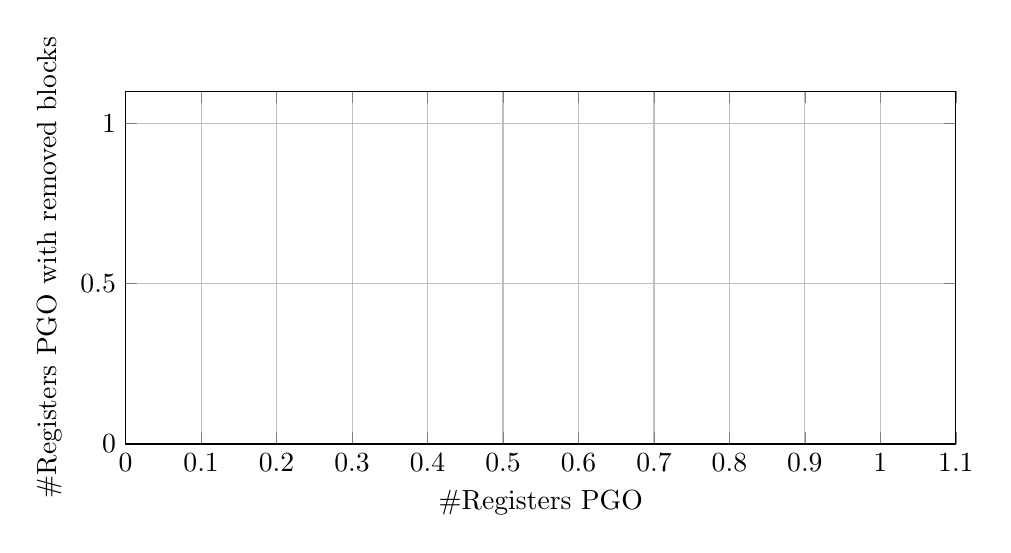
\begin{tikzpicture}
\begin{axis}[
	scatter/classes={
		dota={fill=color0},%
		madmax={fill=color1}},
	xlabel={\#Registers PGO},
	ylabel={\#Registers PGO with removed blocks},
	xmin=0,
	ymin=0,
	grid=both,
	legend style={at={(0,1)},anchor=north west},
]

\runtex{register-scatter}

\draw
(axis cs:\pgfkeysvalueof{/pgfplots/xmin},\pgfkeysvalueof{/pgfplots/xmin}) --
(axis cs:\pgfkeysvalueof{/pgfplots/xmax},\pgfkeysvalueof{/pgfplots/xmax});

\legend{Dota 2,Mad Max}
\end{axis}
\end{tikzpicture}
\captionof{figure}{Vector register usage comparison when removing blocks, each dot represents a shader}
\label{dia:registers_scatter}
\end{figure}


In summary, removing unused code can greatly reduce the register usage for some shaders.
Unused code in general does not seem to be a problem for games, at least not from the perspective of register usage.

\subsection{Uniform Branches}
\label{sub:eval_uniform_branches}
Apart from basic block counters, we also examined the uniformity of certain variables.
One type of variables that we further looked at are branch conditions.
If a condition is uniform, the branch which is guarded by this condition is taken uniformly by the SIMD unit, if the condition is divergent, the unit has to take both branches after each other.

At compile time, a variable can be classified as uniform or as divergent.
If it is classified as uniform, we know that under all possible circumstances, the variable always contains the same value across all lanes.
Usually, such variables are stored in scalar registers and computations on these variables use the scalar unit.
If a variable is classified as divergent, the compiler is not able to proof that the variable always contains the same value on all lanes.
It does not necessarily mean that the variable value differs on multiple lanes at runtime.
Our instrumentation records the behavior at runtime and classifies a variable as \emph{dynamic uniform}, if it always contains the same value on all lanes or as divergent if not.
\emph{Static uniform} variables are the ones where the compiler can proof that they are uniform.

\begin{figure}
\pgfplotsset{width=\textwidth}
\centering
\begin{tikzpicture}
\begin{axis}[
	ybar stacked,
	enlarge x limits=0.2,
	cycle list name=mycolors,
	symbolic x coords={ashes,dota,dow3,f12017,madmax},
	xticklabels={Ashes,Dota 2,Warhammer,F1 2017,Mad Max},
	xtick=data,
	ylabel={Uniformity [\SI{}{\percent}]},
	ymin=0,
	ymax=100,
	grid=both,
	nodes near coords,
	% Do not display text for nodes with value < … by setting opacity to 0
	node near coords style={
		/utils/exec={\setbox0\hbox{\pgfmathprintnumber\pgfplotspointmeta}
		\pgfmathfloattomacro{\pgfplotspointmeta}{\F}{\M}{\E}
		\pgfmathsetmacro{\myopacity}{ifthenelse(\M*pow(10,\E)<17,0,1)}
		},
		rotate=90, anchor=center, opacity=\myopacity},
	bar width=0.5cm,
	legend style={at={(1,1)},anchor=south east},
]

\runtex{uniform-branches}
\legend{Static uniform,Dynamic uniform,Divergent}
\end{axis}
\end{tikzpicture}
\captionof{figure}{Uniformity of branches}
\label{dia:uniform_branches}
\end{figure}


\Cref{dia:uniform_branches} shows us how conditions and branches are divided into the three categories.
The \enquote{best} category are the static uniform branches.
For these branches, the compiler can emit a simple branch instruction and the compiler knows that either all or none of the active lanes will take this branch.
Conditions in the dynamic uniform category represent a branch where the compiler emitted additional code to support divergent branching.
At runtime, this code is not used, the branch is always taken by all lanes uniformly.
The performance wise worst case are divergent branches, in these cases, the compiler emits additional code like in the dynamic uniform case and at runtime, both branches are taken by different lanes, so the SIMD unit needs to execute both parts sequentially.

With respect to the grading of the last paragraph, Ashes and F1 2017 are performing best because most of their branches are statically uniform and only a small fraction is divergent.
We need to take into account though that this is a very coarse look at these games, we do not know the size and performance impact of the divergent branches, also sometimes divergent branches are inevitable.

\subsection{Uniform Loads}
\label{sub:eval_uniform_loads}
Similar to the analysis of uniform conditions in the last section, we analysed \texttt{LoadInstr} instructions in LLVM.
The uniformity of loaded memory values is shown in \cref{dia:uniform_loads}.
It is important to know that the analyzed load instructions do not include buffer loads and image loads which are more complicated to analyze because they are indexed with multiple dimensions, can return multiple dimensions, are connected with a sampler, use mip mapping, etc.
\centering
\begin{tikzpicture}
\begin{axis}[
	ybar stacked,
	enlarge x limits=0.2,
	cycle list name=mycolors,
	symbolic x coords={ashes,dota,dow3,f12017,madmax},
	xticklabels={Ashes,Dota 2,Warhammer,F1 2017,Mad Max},
	xtick=data,
	ylabel={Uniformity [\SI{}{\percent}]},
	ymin=0,
	ymax=100,
	grid=both,
	nodes near coords,
	% Do not display text for nodes with value < … by setting opacity to 0
	node near coords style={
		/utils/exec={\setbox0\hbox{\pgfmathprintnumber\pgfplotspointmeta}
		\pgfmathfloattomacro{\pgfplotspointmeta}{\F}{\M}{\E}
		\pgfmathsetmacro{\myopacity}{ifthenelse(\M*pow(10,\E)<17,0,1)}
		},
		rotate=90, anchor=center, opacity=\myopacity},
	bar width=0.5cm,
	legend style={at={(1,1)},anchor=south east},
]

\runtex{uniform-loads}
\legend{Static uniform,Dynamic uniform,Divergent}
\end{axis}
\end{tikzpicture}


\subsection{Performance}
\label{sub:eval_perf}
In addition to the previous analyses, an important part is of course the performance change when using profile-guided optimizations.
To evaluate the performance of shaders, we run the games in three different configurations:Without any special options, using profile-guided optimizations and using PGO with removing unused basic blocks.
As before, removing blocks is only done for Dota 2 and Mad Max, the other games do not work with the current implementation.
\begin{tikzpicture}
\begin{axis}[
	ybar,
	enlarge x limits=0.1,
	cycle list name=mycolors,
	symbolic x coords={ashes,dota,dow3,f12017,madmax,switch},
	xticklabels={Ashes,Dota 2,Warhammer,F1 2017,Mad Max,Switch vm},
	xtick=data,
	xticklabel style={text width=2cm,align=center},
	ylabel={{\color{tumblue}$\blacktriangleleft$} less is better, Time per frame [\SI{}{\milli\second}]},
	ylabel style={align=center},
	ymin=0,
	grid=both,
	%nodes near coords,
	%every node near coord/.append style={rotate=90, anchor=west},
	bar width=0.3cm,
	legend style={at={(1,1)},anchor=north east, font=\scriptsize},
	point meta=explicit symbolic,
	nodes near coords={\pgfplotspointmeta},
	every node near coord/.append style={yshift=0.2cm, font=\scriptsize},
]

\runtex{performance-presentation}
\end{axis}
\end{tikzpicture}


\begin{table}
	\centering
	\runtex{performance}
	\captionof{table}{Performance of games with PGO}
	\label{tab:performance}
\end{table}

The result is displayed in \cref{dia:performance} and \cref{tab:performance}.
In general, the optimizations did not change the performance by a great amount.
On Ashes and F1 2017 it even had a negative effect, these games got a little slower.
Dota and Mad Max did not show a significant difference.
Warhammer reduced the time per frame from \SI{65.98 \pm 0.18}{\milli\second} to \SI{65.31 \pm 0.13}{\milli\second} with PGO, which is an improvement of \SI{1 \pm 0.4}{\percent}.

The order of basic blocks and other optimizations based on basic block counter seem to have a minor effect on performance.
Removing unused blocks had no effect on the two tested games.

\subsection{Overhead}
\label{sub:overhead}
To find hot paths, the instrumentation inserts counters into some basic blocks of a program. The counters introduce an overhead, compared to a non-instrumented version of the code.
In the case of counting the frequency of basic block executions, the counters themselves are not sensitive to timing and thus not directly influenced by this overhead.
But the code will run slower. In the case of a game, we will observe fewer frames per second than usual.
If the benchmark, that we run with PGO instrumentation, runs for a fixed time, we will get lower basic block frequencies for fewer frames per second.
Therefore, the measured counters may show fewer executions than the actual frequencies that we try to measure.
This effect should not have an impact on the optimization results because the ratio of frequencies stays the same, no matter how fast or slow a game runs.

We measured the overhead for two different games in different configurations: Dota 2 and Ashes of the Singularity. The baseline in \cref{dia:overhead} and \cref{tab:overhead} is a normal run of the game with no counters.
The first tested configuration uses normal add instructions (i.e. no atomics) and increments by one per SIMD unit.
The second and third variant use atomic counters, either incrementing by one on each SIMD lane or once per unit.
All instrumentation was inserted after structurizing the CFG.

As expected, incrementing per lane needs the most time. An atomic add causes less overhead for Dota 2 than the non-atomic version.
The reason is that the non-atomic increment needs a load and a store operation where the atomic version needs only a single memory transaction. The actual addition is computed inside the L2 cache for atomics.
For Ashes of the Singularity, we cannot see much of a difference in performance. The per-lane variant is significantly slower but only by \SI{0.25 \pm 0.06}{\percent}.

\begin{figure}
\centering
\pgfplotsset{width=\textwidth}
\centering
\begin{tikzpicture}
\begin{axis}[
	ybar,
	enlarge x limits=0.2,
	cycle list name=mycolors,
	symbolic x coords={ashes,dota,dow3,f12017,madmax},
	xticklabels={Ashes,Dota 2,Warhammer,F1 2017,Mad Max},
	xtick=data,
	ylabel={\footnotesize {\color{tumblue}$\blacktriangleleft$} Time per frame [\SI{}{\milli\second}], less is better},
	ymin=0,
	grid=both,
	%nodes near coords,
	%every node near coord/.append style={rotate=90, anchor=west},
	bar width=0.5cm,
	legend style={at={(1,1)},anchor=north east},
]

\runtex{overhead -d}
\end{axis}
\end{tikzpicture}
\captionof{figure}{Overhead of BB counters}
\label{dia:overhead}
\end{figure}


Similar to the PGO benchmarks, Ashes shows the smallest difference.

\begin{table}
\centering
\runtex{overhead}
\captionof{table}{Overhead of BB counters}
\label{tab:overhead}
\end{table}

In some cases, it may be necessary to decrease the overhead of basic block counters. For example to use the instrumentation in production environments where high overheads are not acceptable.
Sometimes, the overhead is high enough to trigger timeouts in the GPU driver, leading to game crashes. This is the case for the Infiltrator demo project of the Unreal Engine.

A simple way to decrease the overhead is to switch from atomic counters to non-atomic counting. This is enough to let e.g. the Infiltrator demo start, however it comes with a drawback. Shaders are executed highly parallel, so many instances of a shader will simultaneously access the same memory location of a counter.
These race conditions lead to inaccurate counters. Not only do we get wrong proportions of frequencies, we also have to take into account that not every basic block gets a counter, some frequencies are computed from multiple counters. This leads to cases where basic blocks that are not executed at all at runtime are assigned a counter value of several thousand executions because the counter values used to compute the frequencies are inaccurate.

Another overhead reduction can be achieved by skipping counting on most SIMD units and activate it e.g. only on \SI{5}{\percent} of the units.
This means most executions will skip the increments, having even less overhead than the non-atomic variant while the rest of the executions gives accurate statistics.
A problem with this approach is that (e.g. vertex-) shaders that get executed only a few times, might not land on any of SIMD units where counting is activated and we get no statistics at all for them.
This should only be a small problem because these shaders probably do not account for much of the computation time (as they are executed only a few times) and optimizing them cannot yield big benefits anyway.

A more sophisticated technique that can speed up basic block counting tries to reduce the memory pressure by atomics without falling back to non-atomic counting.
As we know, many atomic operations will simultaneously try to access the same memory location.
We can reduce this pressure if we add multiple memory locations in different cache lanes for the same counter and spread the counting over these locations.
As fewer atomic increments access the same memory, they do not have to wait as long as before and the program execution can continue faster.
In the end, when shutting down the application, we have to add up all duplicated counters.
This happens only once in the end for most applications so it adds not much overhead.
